\documentclass[12pt]{beamer}
\usetheme{Madrid}
\usecolortheme{default}

\usepackage{ragged2e}
\usepackage[utf8]{inputenc}
\usepackage[brazil]{babel}
\usepackage[T1]{fontenc}
\usepackage{amsmath}
\usepackage{amsfonts}
\usepackage{amssymb}
\usepackage{graphicx}
\usepackage{setspace}
\setbeamertemplate{caption}[numbered]
\usepackage{hyperref}
\setbeamercovered{transparent} 
\setbeamertemplate{navigation symbols}{}
\usepackage[table,xcdraw]{xcolor}


\addtobeamertemplate{block alerted}{}{\justifying}

\author[Prof. Fábio Rivas \& Joao Victor]{% 
Fábio Rivas\inst{1} \and Joao Victor\inst{2}}
\title{Triângulos, Ruas e Macarrão: o sabor da desigualdade (triangular)}
\institute[]{% 
  \textsuperscript{1} Professor \\
  \textsuperscript{2} Discente, Licenciatura em Matematica
}
\date{\today} 
\titlegraphic{
\includegraphics[width=0.2\textwidth]{imagens/logo_3.jpg}}

%\subject{}

% ---------------------------------------------------------

\begin{document}
\onehalfspacing 
\justifying 

\begin{frame}
    \titlepage
\end{frame}

\begin{frame}{Sumário}
    \tableofcontents
\end{frame}


\section{Desigualdade}

    \begin{frame}{Desigualdade}
        \begin{alertblock}{Definição - Dicionário Michaelis}
        \justifying
        
            \textbf{(1)} Atributo de pessoas ou coisas distintas; dessemelhança, diferença.\\
            \textbf{(2)} Falta de equilíbrio; disparidade, distância.\\
            \textbf{(3)} Comparação de duas quantidades desiguais, em uma expressão matemática, através de sinais (maior, menor, diferente). \\
        \end{alertblock}

        \pause

        \begin{block}{Aplicação}
            Joao, um amante de pizza, decidiu fazer um rolé gastronômico por Manaus para encontrar a MELHOR pizza de frango com catupiry da cidade!
        \end{block}

        
    \end{frame}

    \begin{frame}{A Grande Descoberta Matemática de Joao}
    
        \begin{columns}
        \begin{column}{0.6\textwidth}
       
            \textbf{Pizzaria A - Ingredientes}

            \begin{enumerate}
                \item 300g de frango temperado
                \item 200g de catupiry cremoso
                \item 150g de molho de tomate caseiro
                \item 100g de mussarela derretida
                \item 50g de milho verde
                \item 30g de azeitonas pretas
                \item 20g de orégano fresco
            \end{enumerate}
        \end{column}

        \begin{column}{0.4\textwidth}
            \centering
            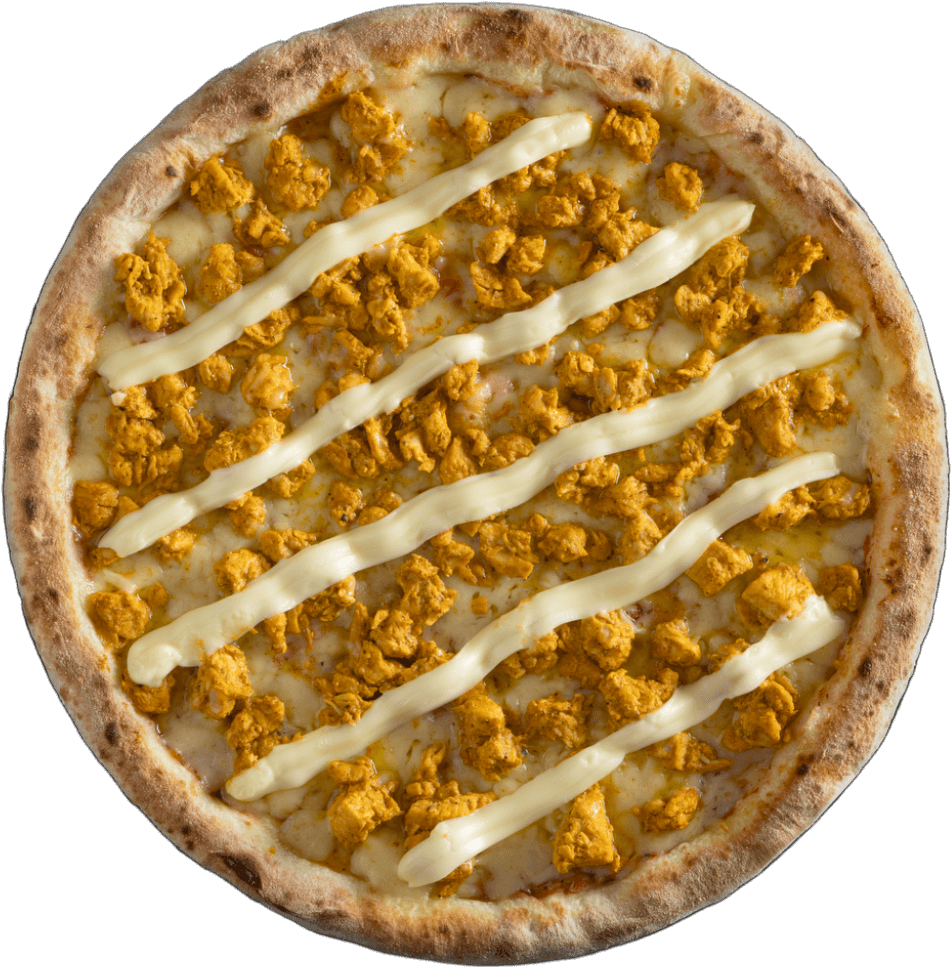
\includegraphics[width=0.8\linewidth]{imagens/pizza_1.png}
        \end{column}
    \end{columns}
        
    \end{frame}

    \begin{frame}{A Grande Descoberta Matemática de Joao}
    
        \begin{columns}
        \begin{column}{0.6\textwidth}
       
            \textbf{Pizzaria B - Ingredientes}

            \begin{enumerate}
                \item 250g de frango temperado
                \item 250g de catupiry cremoso
                \item 120g de molho de tomate caseiro
                \item 120g de mussarela derretida
                \item 40g de milho verde
                \item 30g de azeitonas pretas
                \item 25g de orégano fresco
            \end{enumerate}
        \end{column}

        \begin{column}{0.4\textwidth}
            \centering
            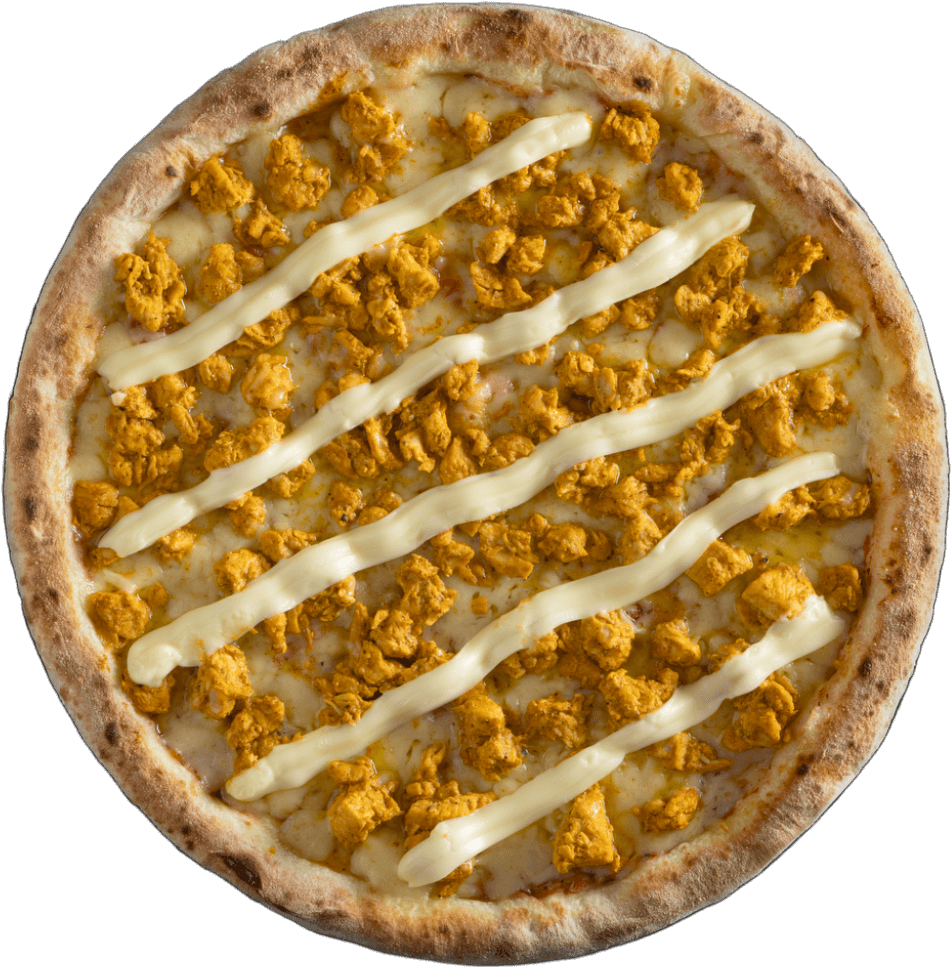
\includegraphics[width=0.8\linewidth]{imagens/pizza_1.png}
        \end{column}
    \end{columns}
        
    \end{frame}
    
    \begin{frame}{Comparando os ingredientes}
    
        \begin{table}[h]
        \centering
        \small
        \renewcommand{\arraystretch}{1.3}
            \begin{tabular}{lccc}
                \hline
                \textbf{Ingredientes (g)} & \textbf{Pizzaria A} & \textbf{Pizzaria B} & \textbf{A vs B} \\
                \hline
                Frango Temperado & 300 & 250 & 50g a mais \\
                Catupiry cremoso & 200 & 250 & 50g a menos \\
                Molho de tomate caseiro & 150 & 120 & 30g a mais \\
                Mussarela derretida & 100 & 120 & 20g a menos \\
                Milho verde & 50 & 40 & 10g a mais \\
                Azeitonas pretas & 30 & 30 & IGUAIS \\
                Orégano fresco & 20 & 25 & 5g a menos \\
                \hline
            \end{tabular}
        \end{table}

    \end{frame}
    
\section{Triângulo}

    \begin{frame}{Triângulo}
        \begin{alertblock}{Definição}
        \justifying
            \textbf{(1)} Polígono de três lados; trilátero.\\
            \textbf{(2)} Qualquer objeto que tenha formato triangular.\\
            \textit{\textbf{(3)} Dados três pontos, A, B e C, não colineares, à reunião dos segmentos $\overline{AB}$, $\overline{AC}$ e $\overline{BC}$, chama-se \textbf{triângulo ABC} (Fundamento de Matemática Elementar, volume 9)}\\
        \end{alertblock}
    \end{frame}

    \begin{frame}{Tipos de triângulos}
        Quanto aos lados, os triângulos se classificam em:

        \begin{center}
            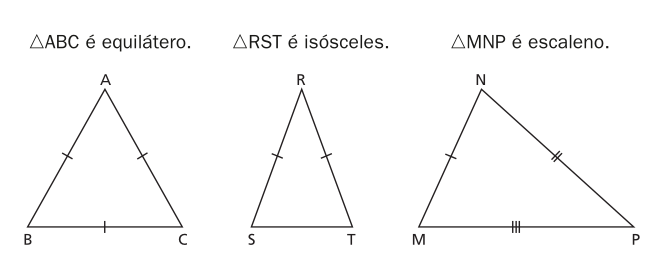
\includegraphics[scale=0.5]{imagens/triangulos.png}
        \end{center}
    \end{frame}
\section{Desigualdade Triangular}

    \begin{frame}{Desigualdade triangular}
        \begin{alertblock}{Definição}
        \justifying
            Em todo triângulo, a soma dos comprimentos de dois lados é maior que o comprimento do terceiro lado. 
        \end{alertblock}
        
        \pause
        
        \begin{block}{Aplicação}
            Existe triângulo cujos lados medem 5, 8 e 16? Por quê?
        \end{block}

    \end{frame}
    
\section{Verificação: é triângulo?}

    \begin{frame}{Aplicação em sala}
        \begin{minipage}{\textwidth}
        \centering
            \fbox{\begin{minipage}{0.9\textwidth}
            \vspace{0.3cm}
            \footnotesize

                \textbf{Como usar:} \\
                1. Escolha 3 palitos e meça seus comprimentos (cada palito = 1 unidade) \\
                2. Anote os valores como a, b, c na tabela \\
                3. Teste cada desigualdade (marque \checkmark\ para Verdadeiro ou $\times$ para Falso) \\
                4. Tente FORMAR o triângulo com os palitos escolhidos \\
                5. Se \textbf{TODAS} as desigualdades forem verdadeiras $\rightarrow$ forma triângulo! \\
                6. Se \textbf{ALGUMA} for falsa $\rightarrow$ não forma triângulo! \\
                \textbf{Regra da Desigualdade Triangular:} \\
                Para formar triângulo: $a + b > c$ \textbf{e} $a + c > b$ \textbf{e} $b + c > a$
                \vspace{0.3cm}
            \end{minipage}}
        \end{minipage}
    \end{frame}

    \begin{frame}{Aplicação em sala}
        \begin{table}[h]
        \centering
        \small
        \setlength{\tabcolsep}{8pt}
        \renewcommand{\arraystretch}{1.5}

            \begin{tabular}{|c|c|c||c|c|c||c|}
                \hline
                \textbf{a} & \textbf{b} & \textbf{c} & \textbf{a + b > c} & \textbf{a + c > b} & \textbf{b + c > a} & \textbf{Triângulo?} \\
                \hline
                & & & $\square$ & $\square$ & $\square$ & \\
                \hline
                & & & $\square$ & $\square$ & $\square$ & \\
                \hline
                & & & $\square$ & $\square$ & $\square$ & \\
                \hline
                & & & $\square$ & $\square$ & $\square$ & \\
                \hline
                & & & $\square$ & $\square$ & $\square$ & \\
                \hline
                & & & $\square$ & $\square$ & $\square$ & \\
                \hline
            \end{tabular}
        \end{table}
    \end{frame}

\section{Problema, probleminhas e \textit{problemão} (OBMEP)}

\begin{frame}{Problema de Gincana: Isso não é perímetro}
    Se $\overline{AB}+\overline{BC}=18$, então o perímetro do triângulo $ABC$ \textbf{NÃO} pode ser:

    \begin{enumerate}[a]
    	\item 33
    	\item 34 
        \item 35
        \item 36 
        \item Nenhuma das respostas anteriores
    \end{enumerate}
\end{frame}



\begin{frame}{Probleminha: Brincando com lápis}
    Ana Paula tinha 2 lápis em mãos, cujos comprimentos eram de 5,8 cm e 11,4 cm, respectivamente. Com esses 2 lápis e um terceiro, entre os que tinha em seu estojo, ela começou a formar triângulos que tivessem os seus lápis como lados. Logo ela percebeu que com alguns dos lápis do estojo não era possível formar um triângulo. 

    \vspace{2mm} 

    Determine para que comprimentos do terceiro lápis Ana Paula conseguirá formar um triângulo.
    
\end{frame}

\begin{frame}{Probleminha: Quem andou mais?}

    Ruas retas e compridas ligam as casas dos amigos Bruno, Francimar e Robério.

    \begin{itemize}
        \item Francimar, em sua caminhada matinal, saiu de sua casa e andou até a casa de Bruno. Em seguida, prosseguiu para a casa de Robério e depois voltou para sua casa.
        \item Mais tarde, Robério, muito concentrado com um problema de matemática, foi até a casa de Bruno e voltou para sua casa.
    \end{itemize} Sem conhecer as distâncias entre as casas, é possível saber quem andou mais?
\end{frame}

\begin{frame}{Problemão: Probabilidade com macarrão}
    Quebrando aleatoriamente um macarrão, de tamanho qualquer, em três partes, qual a probabilidade de que elas possam formar um triângulo?

    \begin{center}
        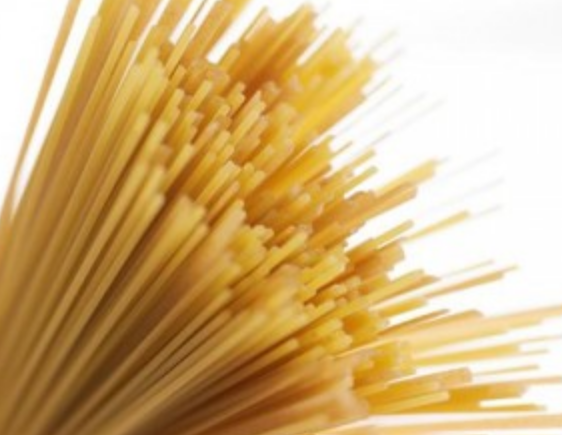
\includegraphics[scale=0.3]{imagens/macarrao.png}
    \end{center}
\end{frame}




\section{Referências}

\begin{frame}{Referências}
	

\end{frame}

\end{document}